\documentclass{article}


\usepackage{arxiv}

\usepackage[utf8]{inputenc} % allow utf-8 input
\usepackage[T1]{fontenc}    % use 8-bit T1 fonts
\usepackage{hyperref}       % hyperlinks
\usepackage{url}            % simple URL typesetting
\usepackage{booktabs}       % professional-quality tables
\usepackage{amsfonts}       % blackboard math symbols
\usepackage{nicefrac}       % compact symbols for 1/2, etc.
\usepackage{microtype}      % microtypography
\usepackage{lipsum}
\usepackage{graphicx}
\graphicspath{ {./images/} }

\usepackage{fontsize}
\changefontsize{11}

\setlength{\parindent}{0pt} % Paragraph indentation
\setlength{\parskip}{1.0em} % Vertical space between paragraphs


\title{Analyse Détaillée de Mixture-of-Recursions (MoE)}


\author{
 Mokira \\
  % School of Coumputing and Information\\
  % University of Pittsburgh\\
  % Pittsburgh, PA 15213 \\
  % \texttt{dr.mokira@gmail.com} \\
  Ingénieur Machine Learning \\
  (+229) 019 798 5109 \\
  \texttt{dr.mokira@gmail.com} \\
  %% \AND
  %% Coauthor \\
  %% Affiliation \\
  %% Address \\
  %% \texttt{email} \\
  %% \And
  %% Coauthor \\
  %% Affiliation \\
  %% Address \\
  %% \texttt{email} \\
  %% \And
  %% Coauthor \\
  %% Affiliation \\
  %% Address \\
  %% \texttt{email} \\
}

\begin{document}
\maketitle
\begin{abstract}
Pourquoi MoR est une petite révolution ?
Imaginez un modèle de langage qui combine l’efficacité mémoire
des architectures à partage de paramètres (comme ALBERT) avec l’intelligence
computationnelle du calcul adaptatif (comme Mixture-of-Depths) :
c’est exactement ce que propose Mixture-of-Recursions (MoR).
Au lieu d’utiliser des couches distinctes, MoR réutilise un même bloc
de calcul de manière récursive, tandis qu’un routeur léger décide
dynamiquement pour chaque mot s’il doit « sortir » rapidement ou "réfléchir"
plus longtemps en passant par des recursions supplémentaires. Résultat ?
Une réduction simultanée de la taille du modèle (-50\% de paramètres),
du temps de calcul (meilleur débit d’inférence) et de la mémoire cache,
sans sacrifier la performance --- ouvrant la voie à des LLMs à la fois agiles,
économiques et puissants. Une avancée architecturale majeure qui mérite
d’être explorée dans les moindres détails !
\end{abstract}


% keywords can be removed
%\keywords{First keyword \and Second keyword \and More}


\section{Introduction}
Aujourd'hui, les intelligences artificielles qui comprennent et génèrent
du langage, comme celles qui animent les assistants virtuels, reposent
sur des architectures dites « Transformers ». Si elles sont impressionnantes,
leur formidable puissance a un coût : une gourmandise excessive en calcul
et en mémoire. Pour fonctionner, ces modèles doivent en effet traiter
chaque mot d'un texte avec la même intensité. Par exemple, pour comprendre
un mot complexe comme « philosophique », un modèle de langue doit lui accorder
autant de temps et de ressources qu’à un mot simple comme « le » ou « et ».
Cette approche uniforme est coûteuse et inefficace.

Les LLMs sont puissants, mais gourmands en mémoire et en calcul.
Et si on pouvait créer un modèle à la fois compact et intelligent,
capable de concentrer ses efforts sur les mots qui en valent vraiment
la peine ?

C'est la réponse à cette question qui a donné naissance
à la \textbf{Mixture-of-Recursions (MoR)}. une nouvelle architecture
qui permet à un modèle de langage d'allouer intelligemment son « effort
de calcul » de manière adaptive, token par token. Imaginez une usine
de traitement où les produits simples sont expédiés rapidement
après une étape, tandis que les produits complexes passent
par plusieurs stations de contrôle pour un travail approfondi.
MoR opère de la même façon : en réutilisant un même groupe de couches
de neurones de manière recursive, et en utilisant un mécanisme de décision
légère pour déterminer quels mots méritent plus de « réflexion ».
Cette méthode unifie pour la première fois les gains en efficacité
mémoire (moins de paramètres) et en efficacité computationnelle
(moins de calculs superflus), sans compromettre les performances.

Dans ce didacticiel, nous commencerons par un rappel des concepts
fondamentaux nécessaires à la compréhension. Ensuite, nous définirons
précisément le problème qui se pose. Puis, nous détaillerons
le fonctionnement de la solution proposée par MoR pour résoudre le problème,
Nous illustrerons cette solution par des exemples concrets
et une implémentation simplifiée en Python.
Nous discuterons ensuite des apports majeurs et des limites de cette solution,
et proposerons des pistes d'amélioration futures,
et enfin conclure sur la portée de ce travail.

\section{Task description and data construction}
\label{sec:headings}
We are provided with five datasets from Kaggle: Sales train, Sale test, items, item categories and shops. In the Sales train dataset, it provides the information about the sales’ number of an item in a shop within a day. In the Sales test dataset, it provides the shop id and item id which are the items and shops we need to predict. In the other three datasets, we can get the information about item’s name and its category, and the shops’ name.
\paragraph{Task modeling.}
We approach this task as a regression problem. For every item and shop pair, we need to predict its next month sales(a number).
\paragraph{Construct train and test data.}
In the Sales train dataset, it only provides the sale within one day, but we need to predict the sale of next month. So we sum the day's sale into month's sale group by item, shop, date(within a month).
In the Sales train dataset, it only contains two columns(item id and shop id). Because we need to provide the sales of next month, we add a date column for it, which stand for the date information of next month.

\subsection{Headings: second level}
\lipsum[5]
\begin{equation}
\xi _{ij}(t)=P(x_{t}=i,x_{t+1}=j|y,v,w;\theta)= {\frac {\alpha _{i}(t)a^{w_t}_{ij}\beta _{j}(t+1)b^{v_{t+1}}_{j}(y_{t+1})}{\sum _{i=1}^{N} \sum _{j=1}^{N} \alpha _{i}(t)a^{w_t}_{ij}\beta _{j}(t+1)b^{v_{t+1}}_{j}(y_{t+1})}}
\end{equation}

\subsubsection{Headings: third level}
\lipsum[6]

\paragraph{Paragraph}
\lipsum[7]

\section{Examples of citations, figures, tables, references}
\label{sec:others}
\lipsum[8] \cite{kour2014real,kour2014fast} and see \cite{hadash2018estimate}.

The documentation for \verb+natbib+ may be found at
\begin{center}
  \url{http://mirrors.ctan.org/macros/latex/contrib/natbib/natnotes.pdf}
\end{center}
Of note is the command \verb+\citet+, which produces citations
appropriate for use in inline text.  For example,
\begin{verbatim}
   \citet{hasselmo} investigated\dots
\end{verbatim}
produces
\begin{quote}
  Hasselmo, et al.\ (1995) investigated\dots
\end{quote}

\begin{center}
  \url{https://www.ctan.org/pkg/booktabs}
\end{center}


\subsection{Figures}
\lipsum[10]
See Figure \ref{fig:fig1}. Here is how you add footnotes. \footnote{Sample of the first footnote.}
\lipsum[11]

\begin{figure}
  \centering
  \fbox{\rule[-.5cm]{4cm}{4cm} \rule[-.5cm]{4cm}{0cm}}
  \caption{Sample figure caption.}
  \label{fig:fig1}
\end{figure}

\begin{figure} % picture
    \centering
    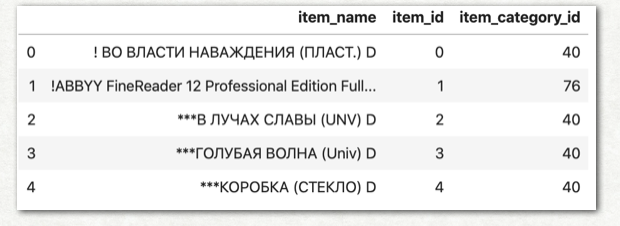
\includegraphics{test.png}
\end{figure}

\subsection{Tables}
\lipsum[12]
See awesome Table~\ref{tab:table}.

\begin{table}
 \caption{Sample table title}
  \centering
  \begin{tabular}{lll}
    \toprule
    \multicolumn{2}{c}{Part}                   \\
    \cmidrule(r){1-2}
    Name     & Description     & Size ($\mu$m) \\
    \midrule
    Dendrite & Input terminal  & $\sim$100     \\
    Axon     & Output terminal & $\sim$10      \\
    Soma     & Cell body       & up to $10^6$  \\
    \bottomrule
  \end{tabular}
  \label{tab:table}
\end{table}

\subsection{Lists}
\begin{itemize}
\item Lorem ipsum dolor sit amet
\item consectetur adipiscing elit.
\item Aliquam dignissim blandit est, in dictum tortor gravida eget. In ac rutrum magna.
\end{itemize}


\bibliographystyle{unsrt}
%\bibliography{references}  %%% Remove comment to use the external .bib file (using bibtex).
%%% and comment out the ``thebibliography'' section.


%%% Comment out this section when you \bibliography{references} is enabled.
\begin{thebibliography}{1}

\bibitem{kour2014real}
George Kour and Raid Saabne.
\newblock Real-time segmentation of on-line handwritten arabic script.
\newblock In {\em Frontiers in Handwriting Recognition (ICFHR), 2014 14th
  International Conference on}, pages 417--422. IEEE, 2014.

\bibitem{kour2014fast}
George Kour and Raid Saabne.
\newblock Fast classification of handwritten on-line arabic characters.
\newblock In {\em Soft Computing and Pattern Recognition (SoCPaR), 2014 6th
  International Conference of}, pages 312--318. IEEE, 2014.

\bibitem{hadash2018estimate}
Guy Hadash, Einat Kermany, Boaz Carmeli, Ofer Lavi, George Kour, and Alon
  Jacovi.
\newblock Estimate and replace: A novel approach to integrating deep neural
  networks with existing applications.
\newblock {\em arXiv preprint arXiv:1804.09028}, 2018.

\end{thebibliography}


\end{document}
